\chapter{実装}
\label{chap:implementation}

本章では第\ref{chap:design}章で述べたシステムの設計を受け、HypAR Touchの実装について述べる。

\newpage

\section{アプリケーション構成}
HypAR TouchはARナビゲーションを表示するモバイルアプリケーション、AR情報やNFC情報を永続化しAPIを提供するサーバー、Scrapbox、Gyazo\footnote{\textsf{TODO:todo}},NFCタグで構成される。(図 \ref{fig:application_structure})

\begin{figure}[h]
  \centering
  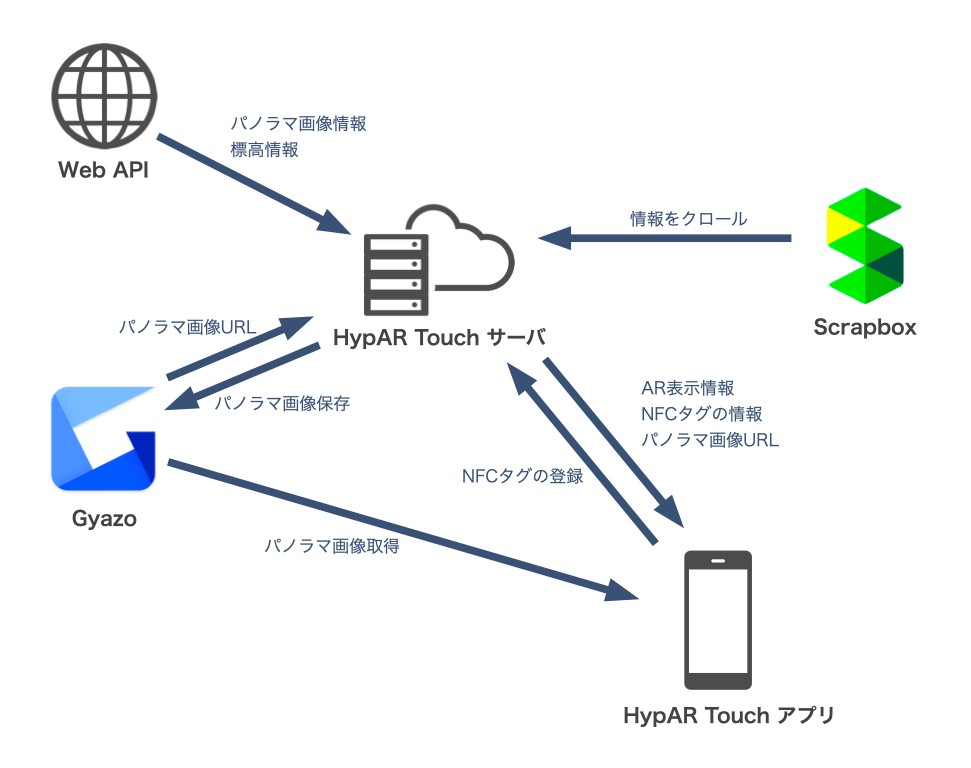
\includegraphics[width=150mm]{images/application_structure.jpg}
  \caption{構成図} \label{fig:application_structure}
\end{figure}

\subsection{HypAR Touchアプリ}
HypAR TouchアプリはReactNative\footnote{\textsf{TODO:todo}}と呼ばれるフレームワークを利用して作成されたモバイル端末アプリケーションである。
ReactNativeを利用することでAndroidとiOSの両方に対応したマルチプラットフォームアプリケーションとなっている。
HypAr TouchアプリはNFCに記録された一意なidを取得し、そのidに紐付いた以下の情報を情報を後述するHypAr Touchサーバーから取得する。
\begin{itemize}
  \item NFCタグの緯度経度
  \item NFCタグの設置される向き(0〜360度)
  \item 表示するAR情報の元となるScrapboxのプロジェクト名
  \item タッチした時に選択されているリンク情報
\end{itemize}
さらに取得したScrapboxのプロジェクトの情報をもとにHypAr TouchサーバーからARで表示する情報を取得し取得する。
最後に取得したARの情報とNFCタグの緯度経度、NFCタグの設置された向きをもとに、各AR情報を表示する相対位置を算出している。
また各AR情報にはそのAR情報付近で撮影されたパノラマ画像のURLが含まれており、移動機能ではこのURLを元に360度画像によるビューを作成している。

\subsection{HypAR Touchサーバ}
HypAR TouchサーバはNode.js\footnote{\textsf{https://nodejs.org/}}上で動作するWebアプリケーションとして実装されている。
HTTPリクエストを処理するWebアプリケーションフレームワークとしてExpress\footnote{\textsf{https://expressjs.com/}}を用い、
そのホスティング環境としてBaaS(Backend-as-a-Service)の一つであるHeroku\footnote{\textsf{https://www.heroku.com/}}を利用している。
HypAR TouchサーバはHypAR Touchアプリで利用するAR情報やNFCタグ情報を管理する役割をもっており、その機能は大きく4つに分けられる。

\begin{itemize}
  \item 対象となるScrapboxのプロジェクトをクロールし、AR表示に必要な情報を整理した上で永続化する。
  
  HypAR Touchサーバは定期的に指定されたScrapboxのプロジェクトをクロールし、位置情報やサムネイル画像のURL、リンク情報などのAR表示に必要な情報をデータベースに永続化している。
  この事によりユーザがScrapboxに加えた変更をARでの表示に対応させることができる。
  \newline

  \item 登録されたNFCタグに関する情報を永続化する。
  
  NFCタグには一意なidがあり、それに紐づく形でタグの位置情報や向き、対象とするScrapboxプロジェクトなどの情報がこのサーバーに記録される。
  \newline

  \item クロールした情報を元にパノラマ画像を生成し、Gyazoに保存した上でそのURLを記録する。
  
  第3章で記述した移動機能を実装するため、ARで表示する情報には記録された位置情報に最も近いところから撮影されたパノラマ画像が必要である。
  そのため HypAR TouchサーバではARで表示する情報全てに対してGoogleStreetView\footnote{\textsf{TODO:todo}}のAPIを利用することでパノラマ画像を生成している。
  また、画像の保存・永続化には後述するGyazoを利用しており、最終的にはGyazoに保存されたパノラマ画像のURLをARで表示する情報と合わせてデータベースに永続化している。
  \newline

  \item 上記3つの情報を取得・追加・変更するAPIを提供する。
  
  HypAR Touchサーバは上記3つの情報を永続化するだけでなく、HypAR TouchアプリからのAR情報取得やNFCタグの登録を受け付ける必要がある。
  そのためHypAR Touchサーバはこれらの情報を取得、追加、更新するAPIを提供している。
  \newline

\end{itemize}

\subsection{Scrapbox}
Scrapboxは第3章で記述したとおり、AR表示するための情報を登録・編集するためのプラットフォームとして利用している。
Scrapboxにはプロジェクト内のページリストと各ページの情報を取得するAPI\footnote{\textsf{https://scrapbox.io/help-jp/API}}を持っており、これを利用することでHypAR Touchサーバのクロールが可能となっている。

\subsection{Gyazo}
Gyazoは、パソコンのデスクトップ画面の一部をキャプチャしてWebにアップロードするツールおよびその画像を保存する画像と映像専用のクラウドストレージサービスである。
Gyazoには画像のアップロード・取得等のAPIが揃っており本システムでのパノラマ画像の保存先として適している。

\subsection{NFCタグ}
本システムで利用するNFCタグはモバイル端末のOSに関わらず、読み込めるタグ形式とデータフォーマットでなくてはならない。
そのため本システムではNFCタグとして最も普及しているISO/IEC 14443 TypeAに準拠したNFCタグを利用している。
また同様にNFC forum\footnote{\textsf{https://nfc-forum.org/}}が策定したデータフォーマットであるNDEF(NFC Data Exchange Format)を利用することでNFC機能を持つ殆どのモバイル端末に対応している。
NDEFのデータ形式には更に細かく、Text、URI、SmartPostermの3つのタイプが存在し、URIタイプで書かれたものは殆どのNFC対応スマートフォンでバックグラウンド読み取りに対応している。
またAndroidとiOSにはディープリンクと呼ばれる特殊なURIからインストールされたアプリケーションを起動する機能が存在しており、そのURIの形式をCustom URL Schemeと呼ぶ。
Custom URL Schemeでは図\ref{fig:custom_url_scheme}のように起動するアプリの指定だけでなく、URIパラメータ利用して追加の情報を指定することが可能である。
このような特徴を踏まえ、本システムではNFCタグにCustom URL Schemeの形にしたURIをNDEFのURIタイプとして記録している。
これにより、でモバイル端末側でNFCタグにタッチするだけでアプリの起動及びtagIDの受け渡しが可能となる。


\begin{figure}[h]
  \centering
  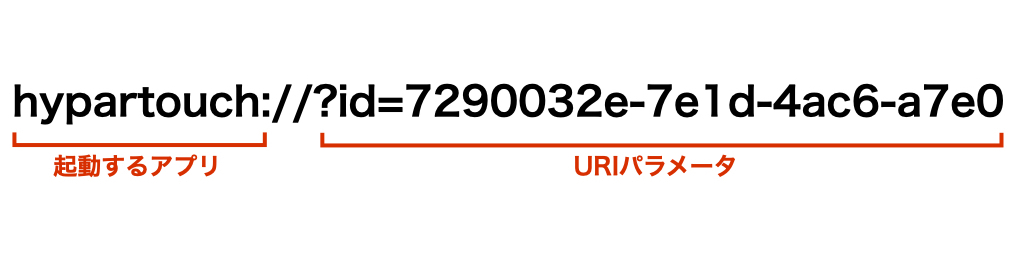
\includegraphics[width=150mm]{images/custom_url_scheme.jpg}
  \caption{Custom URL Scheme} \label{fig:custom_url_scheme}
\end{figure}


\section{NFCによるキャリブレーション}
NFCタグによって行われる位置推定の仕組みについて解説する。
